We have previously defined \textit{TinyFace} as a face detector application, powered by neural networks, and running in a TensorFlow-Lite interpreter environment, where certain steps have been undertaken to reduce model size and complexity. This chapter will present a working application where this has been made possible. \par
As previously discussed, there are esentially 4 steps to building \textit{TinyFace}: gathering data, experimenting with convolutional neural-network model architectures, training, and, finally, evaluating inference performance. With it being an iterative process, this means that after running through all 4 steps, we must go back to step 1 and try improving our model's performance even more. \par

\section{Webscrapper}
\subfile{tables/datasets_2}
Webscrapper is a Selenium-based automatic web-scraping tool, which can search for, download, pre-process, crop and add custom or random side-paddings, sort and categorize, filter and save images where faces are present. We need Webscapper to build datasets for training, but we will not go into more detail about it. Some examples of custom-generated datasets that were used by the author during training, as well as the shape of their contents can be seen in \textit{Table \ref{tab:numpy_training_shape}}. The best performance was achieved using \textit{Own Dataset 3}. \par
Another aspect that has impacted the accuracy of the trained model was the amount of padding (background left intact around the face) and the place where it was applied (i.e. if the images were centered relative to the face or if they had been intentionally skewed to one side). In \textit{Table \ref{tab:numpy_training_padding}} we can see several different datasets of size 30,000 with side dimensions of 100*100, and the amount of (randomized - i.e. not equal on the two different sides, but randomly distributed and intentionally made uneven) padding aroud the image. This skewed padding gives us more realistic images.
\begin{figure*}[ht!]
    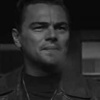
\includegraphics[width = 2 cm]{images/leo/3c5d0190660}\hfill
    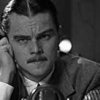
\includegraphics[width = 2 cm]{images/leo/3e3f6a53350}\hfill
    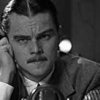
\includegraphics[width = 2 cm]{images/leo/3e3f6a53350}\hfill
    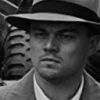
\includegraphics[width = 2 cm]{images/leo/3f4b0e0c760}\hfill
    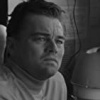
\includegraphics[width = 2 cm]{images/leo/4b605e33360}\hfill
    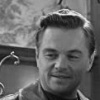
\includegraphics[width = 2 cm]{images/leo/24eb14f9da0}\hfill
    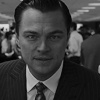
\includegraphics[width = 2 cm]{images/leo/188d3b34ff1}\hfill
    \caption{Training images with randomized side paddings}
\end{figure*}

\section{Compressed Squeezenet}
\subsection{Goals}
Having resolved to formalize the training and evaluation of models, several Python scripts have been written to automate this task. Thus, we firstly needed to write up all the identified model candidates in TensorFlow, in order to be able to call them up for training. This was done for all 4 models from the previous chapter. After training and evaluating performance, the best accuracy and also the smallest size were achieved by Squeezenet.
\subsection{Architecture}
We have settled on a modified Squeezenet-type model architecture. In \textit{Figure \ref{netron_sqnet}} we can find a fully expanded description of the trained and quantized model architecture, in graph form. In essence, we just need to remember from the previous chapter that the model comprises of several fire layers, which come one after the other in sequential order. We should note that the operation \textit{FakeQuant} is still not entirely supported by the stable channel implementations of the TFLite interpreter.

\begin{figure}[!tbp]
\centering
\subfloat[Top Third]{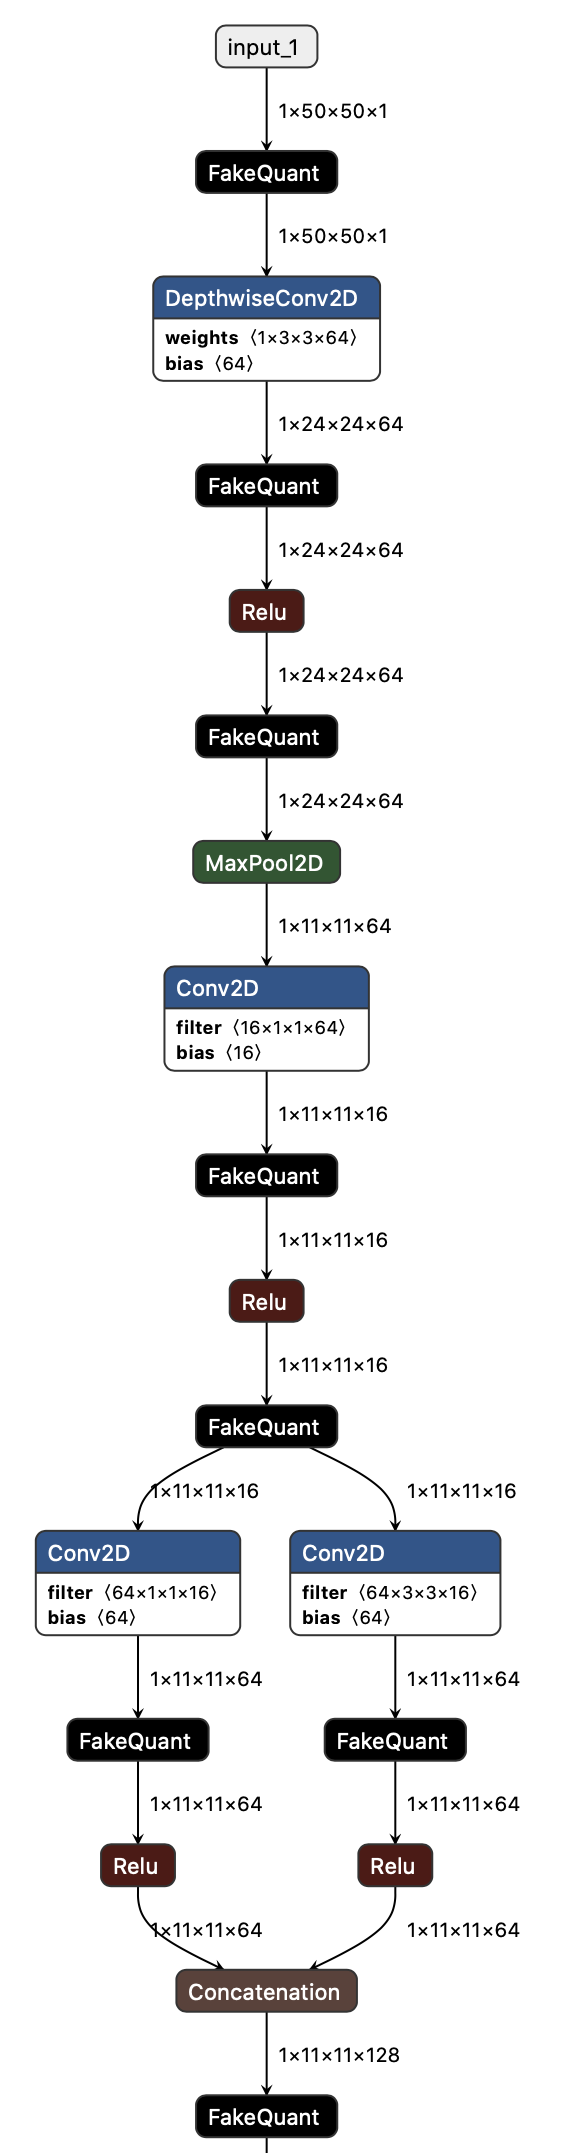
\includegraphics[height = 20 cm]{images/netron_sqnet_1.png}
\label{fig:f1}}
\hfill
\subfloat[Middle Third]{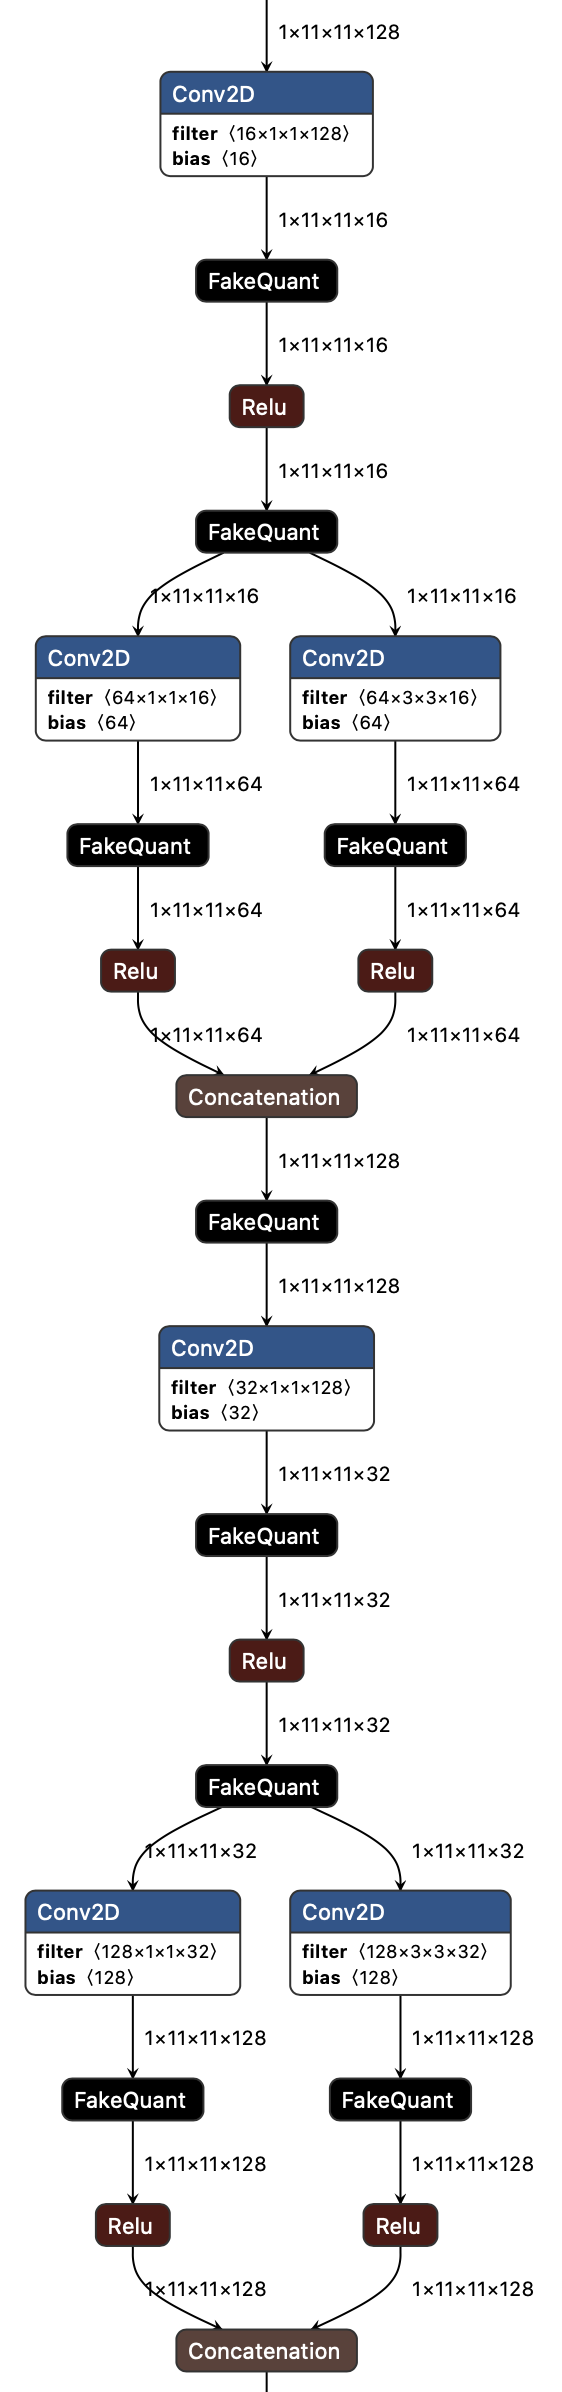
\includegraphics[height = 20 cm]{images/netron_sqnet_2.png}
\label{fig:f2}}
\subfloat[Bottom Third]{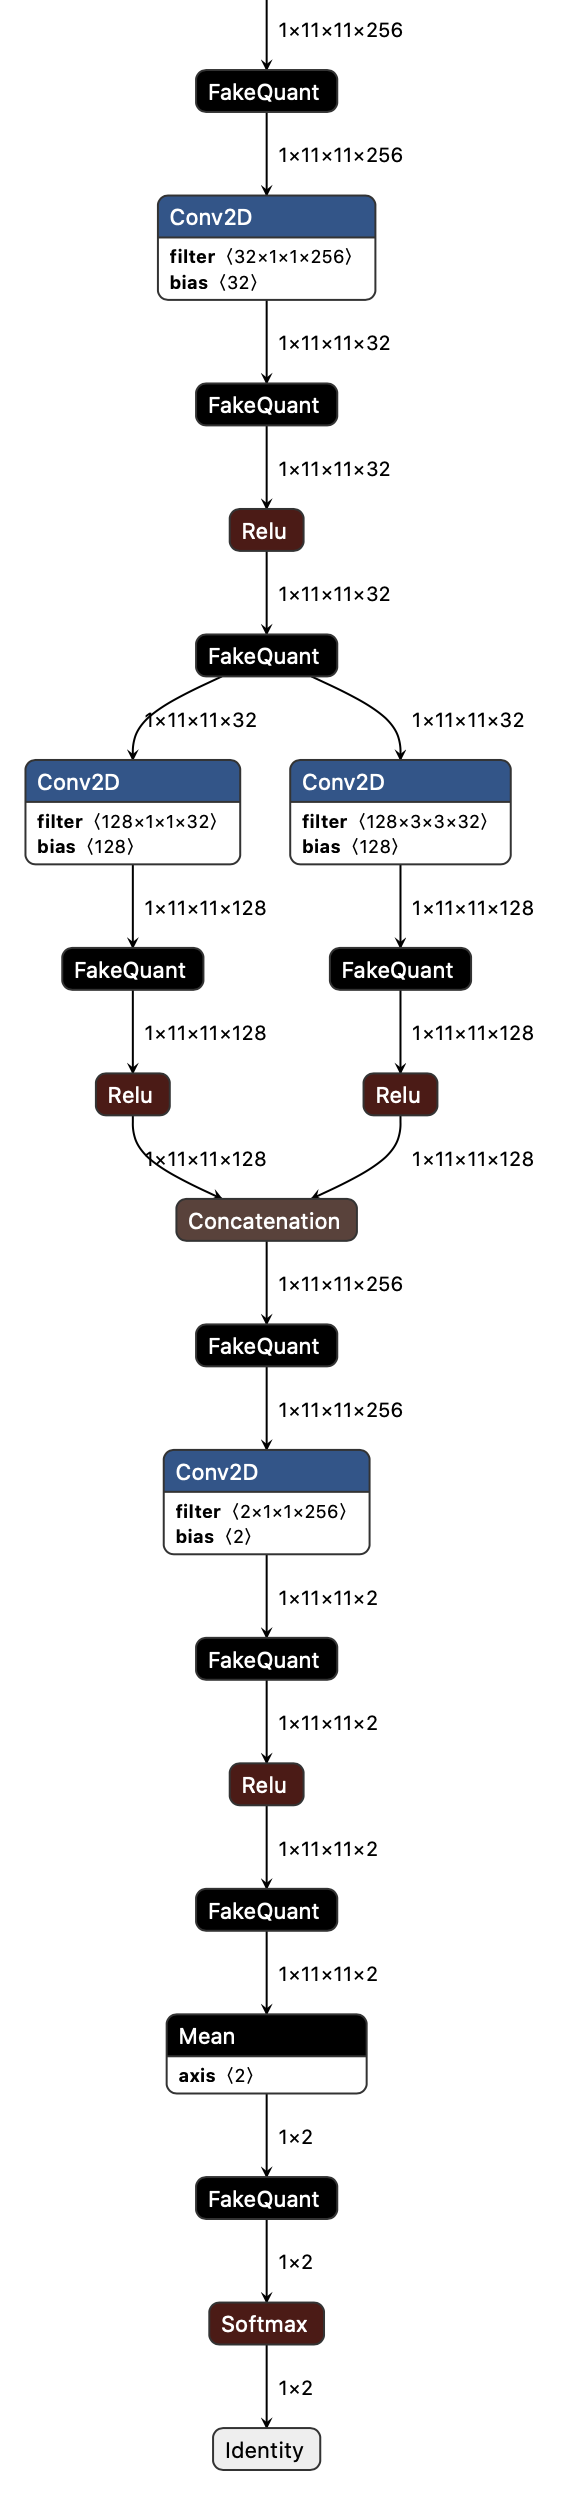
\includegraphics[height = 20 cm]{images/netron_sqnet_3.png}
\label{fig:f3}}
\caption{Expanded view of trained and quantized Squeezenet. Note that the image was divided so it would fit on one page. Generated from TF-Lite file by Netron. \cite{netron}}
\label{netron_sqnet}
\end{figure}

\section{The Model Trainer}
\subsection{Purpose}
This script handles loading training data into memory, configuring the models for training (e.g. parsing the correct image dimensions, by inspecting the loaded images) and, if needed, adapting the training data if the format is not completely correct for our purposes (e.g. color ranges vary - we often need to normalize images to a smaller dynamic range), calling the desired model, applying the needed quantization and compression steps, as well as delivering training metrics afterwards to help us evaluate accuracy. 
\subsection{Code Architecture}
The script esentially calls 3 different methods to accomplish the above described task. 
\begin{enumerate}
    \item \textbf{load\_dataset}: searches the path for each individual image file, loads it and its label, shuffles images and generated extra data by means of data augmentation - we have determined that this improves the final model accuracy. 
    \item \textbf{run\_training}: compiles (\textit{builds}) the model, applies quantization and compression and starts training. Afterwards, it calls upon the \textit{history} generator to give us an overview of the training process.
    \item \textbf{summarize\_diagnostics}: uses \textit{pyplot} to represent the training analytics as plots.
\end{enumerate}
We can also see the code structure in \textit{Figure \ref{xcode_struct}}.

\begin{figure}
    \centering
    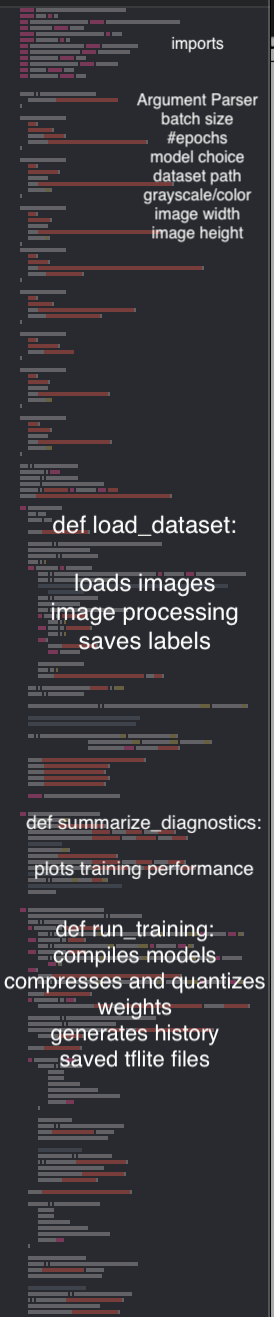
\includegraphics[height = 20 cm]{images/code_body_xcode.png}
    \quad
    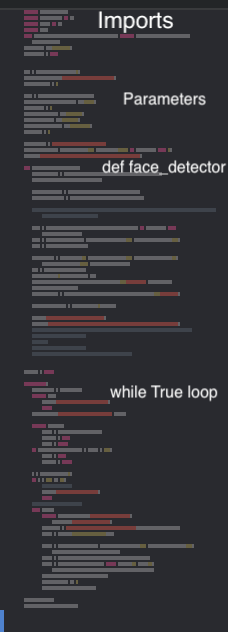
\includegraphics[height = 18 cm]{images/code_body_xcode_webcam.png}
    \caption{Code structure of the model trainer and the webcam app}
    \label{xcode_struct}
\end{figure}

\section{The Webcam App and Inference}
This is the live-demo type, model compiler-based, application where we can put the trained model to the test in real-life, by calling a model interpreter over an image from our webcam. We also have the option to load an image from a local file and run inference on it. 
\subsection{Code Structure}
This application uses OpenCV to parse the webcam into image files in real-time, which can then be given to the model interpreter as numpy arrays to perform inference on. There are esentially 2 parts to this program: a method called \textit{face\_detector}, which includes the TensorFlow code for instantiating the model and running inference and a \textit{while True} loop which polls the webcam and passes the input to the above named method. The code structure is again presented in \textit{Figure \ref{xcode_struct}}. There is not much image processing involved, we just crop the image to the desired square shape, turn it grayscale (from color) and normalize the dynamic range to a range of 0-10.
\subsection{Inference Performance}
Calling the model statically over any image from the dataset will generally result in a perfect result - we can assume 99\% accuracy. This is also the case for 85-90\% of other well-lit and well-centered images, which had not been used for training, where the faces are clear and facing the camera. However, we must note that these are mostly images of actors either in movie scenes or at movie-related events. This means most images are not direct \textit{mug-shots} of faces with uniform backgrounds, as an image from the webcam would be. This translates to the model behaving slightly differently with the webcam app. We have found that it \textit{actually helps} the model in terms of accurately identifying our face if we tilt our head slightly to the side or find a non-uniform background to set ourselves in front of. Smiles tend to sometimes help, too - most training images feature smiling faces, after all, and removing glasses is also very helpful. 